\section{Foursquare}
\label{section:data-foursquare}
\label{section:foursquare}
Trip distribution models that consider only population and employment have a significant flaw. They fail to account attractions, such as national parks that draw large numbers of people, yet exist in areas of low population and employment. Discrete choice modeling provides the opportunity to incorporate parameters that reflect these drivers of travel demand. 
	
Leisure travel is a particular case where socioeconomic metrics don't always reflect the attractiveness of a destination. Areas such as as lakes, national parks and ski resorts are popular long distance recreational destinations in the summer and winter respectively, yet have small populations and employment. 
	
The TSRC microfile records the activities performed on each recorded trip and destination visited during a trip. When aggregated by trip destination, these activities give an indication of which zones provide particular attractions such as national parks or ski areas. The number of trips with each recorded activity can also be used to identify the importance of a particular activity for each zone. However, there are two key problems with this approach:

\begin{itemize}
\item When implementing the model, the spatial resolution of the TSRC microfile means that the location where an activity was performed can only be determined at a zone level. Another data source is still needed to identify key points of interest such as hospitals and tourist attractions to predict trip destinations at the TAZ level.
\item As a domestic survey, the TSRC doesn't cover the US, meaning a different method would need to be used to identify key attractions across the border.
\end{itemize}	
In this section, we describe how the collection and processing of foursquare check-in data was performed in order to build destination utility variables.

\subsection{Foursquare venue search API}
Foursquare collects a wealth of data, on where and when users check-in. Users and their behavior can be tracked over time using twitter as a proxy, however the time-frame for this thesis made this method unfeasible. Instead, the public venue API was used, which is much more limited in its scope, only providing a cross-sectional dataset of POIs within the search area. For a search area and criteria, the API returns a list of venues in JSON format. Each venue record provides the following relevant information:
\begin{itemize}
\item Name
\item Venue category
\item Geo-referenced location
\item Number of unique visitors
\item Number of total check-ins
\end{itemize}

Each request is limited to roughly 1 square degree of longitude and latitude in search area, and only the top 50 venues for that search are returned. A limit of 5000 requests per hour is also enforced. Search results are returned based on the popularity of the venues. How the rank of returned venues is determined by foursquare is not specified. 

The API does not return check-in counts by date, so it can only be used to generate a total metric of activity for each venue, up to the time of the search. For the forecasting of trips to individual venues, this would present a significant obstacle. In this thesis, however, the foursquare metrics are only used for identifying the intensity of activity in zones that may not be reflected in socioeconomic variables. Check-in counts also can not be filtered by origin country or state. This capability would, in a larger model, also allow us to identify U.S. destinations that are commonly visited by Canadian travelers, as opposed to all users of foursquare.

\subsection{Demographic bias}
While the use of social networks is becoming more ubiquitous throughout the general population, LBSNs such as foursquare still have a particular user demographic, which should be taken into account when working with social network based data. The data retrieved from the foursquare API does not provide any demographic information that can be used to weight the retrieved data.

In this thesis, the potential impact of bias is minimized, as only the intensity of activity for each category in a zone is measured as a variable. There is also no stratification of these variables by age, gender or education level in the model estimation. Such stratification would cause concerns with demographic bias, for example with older groups of travelers. One concern is that certain venue categories could be under-represented in the data, such as aged-care services, or those where a check-in might be taboo such as a place of worship. This is considered by grouping venues into broad categories, which are then considered as model parameters.
	
\subsection{Methodology}
To collect the venue data from the Foursquare API, the following procedure was followed:
\begin{enumerate}

\item A developer account was set up to access the API. 
\item The maximum search area allowed is smaller than most external zones, so a search grid of 1 degree raster cells was generated for the study area. 

\item Using the activities specified in the TSRC as a reference, a selection of potentially important venue categories was curated (see table~\ref{table:foursquare_categories}).

\item Each category was mapped to at most 5 main foursquare venue categories, on which the search was performed. This is necessary to exclude venue categories such as ``States \& Municipalities".

\item A python script was written to query the foursquare API for each raster cell and category, returning the top 50 venues, while adhering to the rate limit of 5000 requests per hour. Calls to the api had to be structured as:
\begin{verbatim}
https://api.foursquare.com/v2/venues/search?intent=browse
    &limit=50&sw={sw}&ne={nw}& categoryId={categories}
\end{verbatim}
where 
\begin{itemize}
\item sw, ne are the bottom-left and top-right corners of the search area
\item categories is a comma separated list of venue ids.
\end{itemize}

\item Unique venues were then stored in the PostGIS database, and each tagged with the zone to which it geographically belongs.
\item Two attributes were then calculated for each zone and category; the number of venues of that category in the zone, and the number of check-ins for each category and zone.
\end{enumerate}

A correlation analysis of the created variables shows a high correlation between them (see figure~\ref{fig:foursquare-correlation}. However, this would not be the case if aggregation was performed at the TAZ level. It is still worth investigating the usefulness of these variables in the model estimation, as the number of variables increases the applicability of the model to scenario analysis.  The scenario analysis in section~\ref{scenario-analysis} demonstrates that a model based on these variables produces reasonable results, despite the correlation between the variables.

The foursquare API provides data at a higher spatial resolution than the TSRC microfile, but without the temporal detail. In table~\ref{table:foursquare_categories}, the number of venues and check-ins per category are presented. In total, 34,041 unique venues and 7,981,458 check-ins were collected for the different categories.
\begin{figure}[H]
\centering
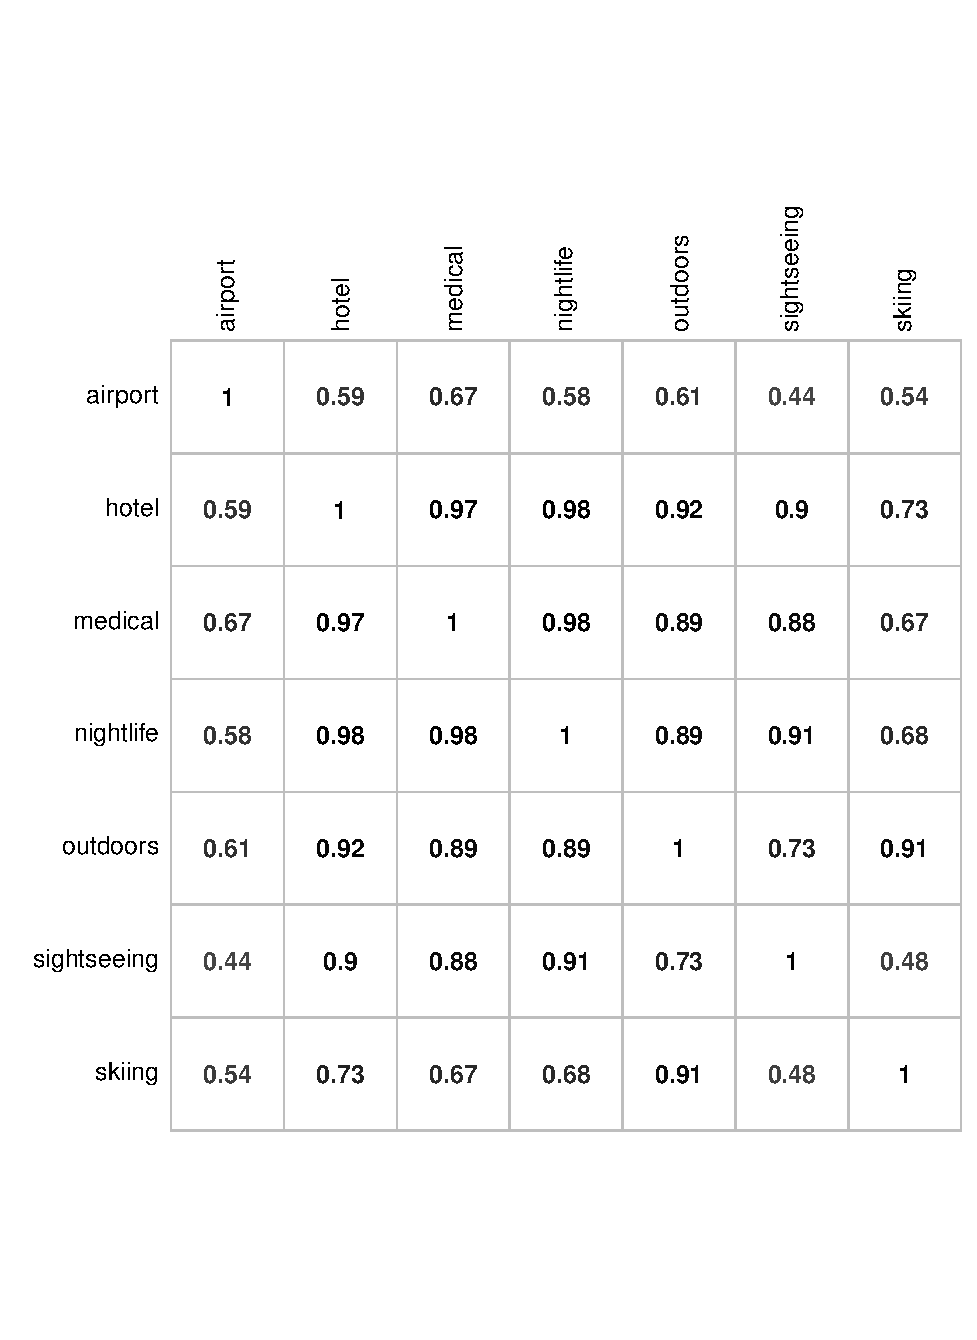
\includegraphics[width=\textwidth]{foursquare_correlation}
\caption{Correlation of foursquare categories between destination zones}
\label{fig:foursquare-correlation}
\end{figure}



%\afterpage{%
%    \clearpage% Flush earlier floats (otherwise order might not be correct)
%    \thispagestyle{empty}% empty page style (?)
%    \begin{landscape}% Landscape page

% Please add the following required packages to your document preamble:
% \usepackage{booktabs}
\begin{sidewaystable}[]
\centering
\caption{foursquare venue categories}
\label{table:foursquare_categories}

\centering % Center table

% Table generated by Excel2LaTeX from sheet 'Sheet1'
% Table generated by Excel2LaTeX from sheet 'Sheet1'
\begin{tabular}{lrrrrrrr}
\toprule
Search Category & \multicolumn{5}{c}{Venue Categories}  & \multicolumn{1}{l}{Venues} & \multicolumn{1}{l}{Check-ins} \\
\midrule
Medical & \multicolumn{1}{l}{Dentist's Office} & \multicolumn{1}{l}{Doctor's Office} & \multicolumn{1}{l}{Hospital} & \multicolumn{1}{l}{Medical Center} & \multicolumn{1}{l}{Veterinarian} &          6,294  &              586,082  \\
Ski Area & \multicolumn{1}{l}{Ski Area} & \multicolumn{1}{l}{Ski Chairlift} & \multicolumn{1}{l}{Ski Chalet} & \multicolumn{1}{l}{Ski Lodge} & \multicolumn{1}{l}{Ski Trail} &          1,048  &              203,266  \\
Airport & \multicolumn{1}{l}{Airport} & \multicolumn{1}{l}{Airport Gate} & \multicolumn{1}{l}{Airport Lounge} & \multicolumn{1}{l}{Airport Terminal} & \multicolumn{1}{l}{Plane} &          1,882  &          1,919,050  \\
Hotel & \multicolumn{1}{l}{Bed \& Breakfast} & \multicolumn{1}{l}{Hostel} & \multicolumn{1}{l}{Hotel} & \multicolumn{1}{l}{Motel} & \multicolumn{1}{l}{Resort} &          7,268  &          1,502,248  \\
Nightlife & \multicolumn{1}{l}{Bar} & \multicolumn{1}{l}{Brewery} & \multicolumn{1}{l}{Dive Bar} & \multicolumn{1}{l}{Pub} & \multicolumn{1}{l}{Sports Bar} &          5,900  &          1,936,153  \\
Outdoors & \multicolumn{1}{l}{National Park} & \multicolumn{1}{l}{Campground} & \multicolumn{1}{l}{Nature Preserve} & \multicolumn{1}{l}{Other Great Outdoors} & \multicolumn{1}{l}{Scenic Lookout} &          7,262  &              709,274  \\
Sightseeing & \multicolumn{1}{l}{Art Gallery} & \multicolumn{1}{l}{Historic Site} & \multicolumn{1}{l}{Museum} & \multicolumn{1}{l}{Theme Park} & \multicolumn{1}{l}{Scenic Lookout} &          4,387  &          1,125,385  \\
\midrule
Total &       &       &       &       &       &       34,041  &          7,981,458  \\
\end{tabular}%

\end{sidewaystable}

%\end{landscape}
%\clearpage% Flush page

